\chapter{Ergebnisse}
Die Ergebnisteil kann sich in (1) Beschreibung der Ergebnisse ohne Vorgriff auf die Interpretation oder Diskussion sowie (2) ggf. in die Darstellung der in der Untersuchung erhobenen Ergebnisse in anschaulicher Form (z. B. Tabellen, Abbildungen) gliedern. Es empfiehlt sich häufig eine dreistufige Vorgehensweise:
\begin{enumerate}
	\item deskriptive Statistik (zur Beschreibung der abhängigen oder unabhängigen Variable für die gesamte Stichprobe)
	\item Inferenzstatistik (Hypothesentestung, z. B. getrennt nach unabhängigen Variablen)
	\item weiterführende Analysen (z. B. Prüfung des Einflusses von Kontrollvariablen oder des Zusammenhangs von abhängigen Variablen)
	Zur besseren Veranschaulichung können Abbildungen wie folgt verwendet werden:	
\end{enumerate}
\begin{figure}[h]
	\centering
	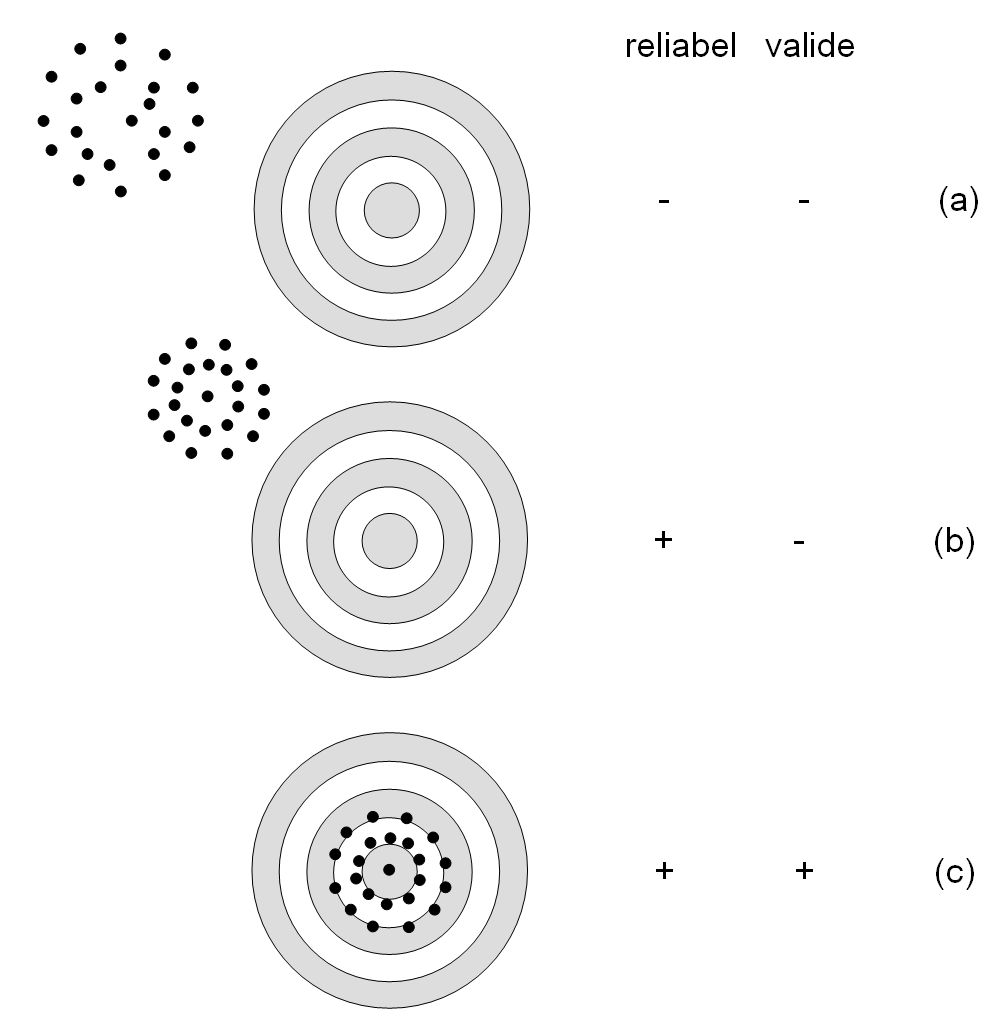
\includegraphics[width=0.7\linewidth]{images/guetekriterien-reliabilitaet-und-variabilitaet}
	\caption{Verdeutlichung der Gütekriterien Reliabilität und Validität~\parencite[23]{Boes2004}.}
	\label{fig:guetekriterien-reliabilitaet-und-variabilitaet}
\end{figure}
Tabellen werden dagegen so verwendet:
\begin{table}[h]
	\centering
	\caption{Übersicht über die wichtigsten Abkürzungen für das Literaturverzeichnis (mod. nach~\cite[9]{DVS2013}).}
	\label{tab:uebersicht-wichtigste-abkuerzungen}
	\begin{tabular}{|c|c|c|c|}
		\hline
		Begriff & deutschsprachiges Werk & \multicolumn{2}{c|}{englischsprachiges Werk}\\
		\hline
		Herausgeber & Hrsg. & Ed. (editor) & Eds. (editors) \\
		\hline
		Seite & S. & p. (page) & pp. (pages) \\
		\hline
	\end{tabular}
\end{table}
